%%%%%%%%%%%%%%%%%%%%%%%%%%%%%%%%%%%%%%%%%%%%%%%%%%%%%%%%%%%%%%%%%
%%% %
%%% % weiiszablon.tex
%%% % The Faculty of Electrical and Computer Engineering
%%% % Rzeszow University Of Technology diploma thesis Template
%%% % Szablon pracy dyplomowej Wydziału Elektrotechniki 
%%% % i Informatyki PRz
%%% % June, 2015
%%%%%%%%%%%%%%%%%%%%%%%%%%%%%%%%%%%%%%%%%%%%%%%%%%%%%%%%%%%%%%%%%

\documentclass[12pt,twoside]{article}

\usepackage{weiiszablon}
\usepackage{csquotes}

\author{Łukasz Miłoś}

% np. EF-123456, EN-654321, ...
\studentID{EF-161883}

\title{System zarządzania bazą BOM}

%%% wybierz rodzaj pracy wpisując jeden z poniższych numerów: ...
% 1 = inżynierska	% BSc
% 2 = magisterska	% MSc
% 3 = doktorska		% PhD
%%% na miejsce zera w linijce poniżej
\newcommand{\rodzajPracyNo}{0}

%%% promotor
\supervisor{(dr inż.) Mariusz Borkowski (prof. PRz)}
%% przykład: dr hab. inż. Józef Nowak, prof. PRz

%%% promotor ze stopniami naukowymi po angielsku
\supervisorEN{(EngD) Mariusz Borkowski}

\begin{document}

% strona tytułowa
\maketitle
\blankpage

% spis treści
\tableofcontents
\clearpage
\blankpage

\section{Wstęp}
Projekt dotyczy przedmiotu \enquote{Usługi sieciowe w biznesie} i zgodnie z założeniami ma ściśle praktyczny charakter.

Sam przedmiot skupia się na zagadnieniach informatyzacji w przedsiębiorstwach, które wpływają na ich organizację i strukturę. Dzięki zastosowaniu różnej klasy systemów, działania ludzkie są wspierane, a często także zastępowane poprzez wykorzystanie nowych technologii, co ma swoje odzwierciedlenie w większej wydajności, produktywności, mniejszym ryzyku popełnienia błędu, a co za tym idzie także minimalizacji kosztów operacyjnych. Wiele zagadnień w przedsiębiorstwach można ułatwić poprzez zastosowanie odpowiedniego systemu zintegrowanego, stąd niezbędna wiedza o typach, funkcjach i przypadkach użycia poszczególnych technologii.

Spośród mnogości zagadnień wybrano temat dotyczący organizacji zasobów produkcyjnych, jako bardzo istotny element wielu przedsiębiorstw.

W ramach projektu utworzono system zarządzania bazą BOM (Bill of Materials). Zagadnienie to jest ściśle związane z przedmiotem i zostanie opisane w kolejnym rozdziale.

\clearpage

\section{Opis problemu}

BOM (Bill Of Materials) jest strukturalnym (hierarchicznym) zestawieniem materiałowym produktu końcowego zawierającym listę części składowych niezbędnych do jego wytworzenia wraz z podaniem cech określających dany zasób m.in. ceny i ilości. Takie zestawienia są wykorzystywane na różnych etapach produkcji, zarówno podczas projektowania, a także podczas wytwarzania czy nawet montażu.

Niekiedy BOM jest wzbogacany o opis kolejnych czynności, w których używane są poszczególne elementy składowe (przykładem jest dowolna instrukcja szafy przeznaczonej do samodzielnego montażu, która często zawiera elementy składowe wraz z wyszczególnieniem kolejnych czynności montażowych).

Poszczególne elementy posiadają kilka cech (atrybutów). W zależności od implementacji systemu parametry są różne. Oto kilka najpopularniejszych z nich:

\begin{itemize}[label=-,labelsep=0.4cm,leftmargin=0.6cm]
\item nazwa
\item identyfikator
\item ilość
\item jednostka miary
\item cena jednostkowa
\item cena sumaryczna
\end{itemize}

Wyjściowym etapem w konstrukcji zestawienia materiałowego może być ogólne, koncepcyjne przedstawienie części składowych produktu finalnego, tak jak pokazano na przykładzie poniżej.

\begin{figure}[ht]
	\centering
	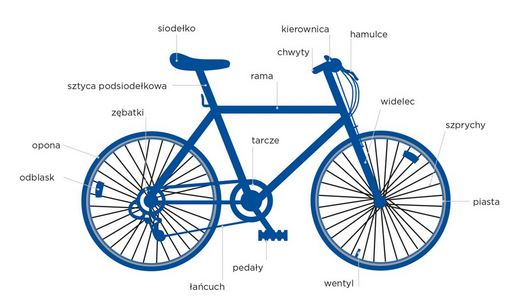
\includegraphics[width=\textwidth]{figures/examples/bicycle.jpg}
	\caption{Przykład koncepcyjnego zestawienia BOM dla roweru [https://www.mecalux.pl/blog/zestawienie-materialowe-bom]}
\label{fig:example:bicycle}
\end{figure}

Należy zwrócić uwagę, że poszczególne elementy składowe, także składają się z mniejszych elementów składowych. Ważne jest dojście do odpowiedniego stopnia złożoności, który zależy od specyfiki danego przedsiębiorstwa. Przykładowo dla firmy produkującej rowery, powyższy schemat (\ref{fig:example:bicycle}) może okazać się wystarczający, jeśli korzysta ona z gotowych produktów innych firm. Przykładem jest tutaj hamulec. O ile firma zakupuje gotowe hamulce od innej firmy i tylko montuje je w swoich rowerach to ten poziom wyszczególnienia jest wystarczający. Natomiast w przypadku produkcji hamulców na własną rękę należałoby dodatkowo wyszczególnić części składowe hamulca (m.in rączka, mocowanie, śruby mocujące, linka, gumki ścieralne, gumki ochronne itd.).


Powyższy schemat jest tylko konceptem. W rzeczywistości zestawienia materiałowe przyjmują formę hierarchii lub tabeli, z wyszczególnieniem poszczególnych elementów, np.

\begin{figure}[ht]
	\centering
	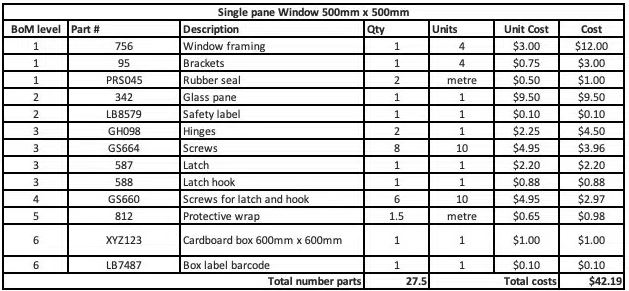
\includegraphics[width=\textwidth]{figures/examples/table.jpg}
	\caption{Przykład zestawienia BOM w formie tabeli [https://www.unleashedsoftware.com/blog/everything-you-need-to-know-about-bill-of-materials]}
\label{fig:example:table}
\end{figure}

Powyżej (\ref{fig:example:table}) przedstawiono zestawienie materiałowe innego produktu w formie tabeli. Niestety wykorzystanie tabeli nie przedstawia wprost hierarchii poszczególnych komponentów. Hierarchia jest tutaj oznaczona za pomocą pierwszej kolumny (BoM level). Powyższe zestawienie (\ref{fig:example:table}) zawiera identyfikator części, opis, ilość, jednostkę, koszt jednostkowy i koszt całościowy. Warto także zwrócić uwagę na podsumowanie zawierające sumę ilości poszczególnych części, a także sumę kosztów.

Najlepszym sposobem prezentacji zestawienia materiałowego (BOM) jest pokazanie hierarchii, np. za pomocą drzewa hierachicznego (treeview), tak jak poniżej.

\begin{figure}[ht]
	\centering
	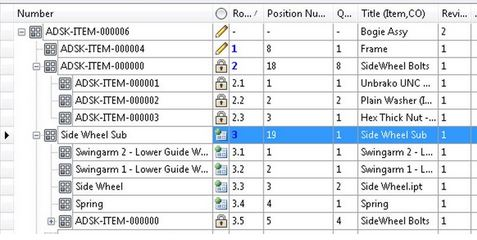
\includegraphics[width=\textwidth]{figures/examples/hierarchy.jpg}
	\caption{Przykład zestawienia BOM w formie drzewa hierarchicznego [https://underthehood-autodesk.typepad.com/blog/items/page/2/]}
\label{fig:example:hierarchy}
\end{figure}

Na rysunku (\ref{fig:example:hierarchy}) widać hierachię. Jest także możliwość rozwijania i zwijania poszczególnych elementów składowych, co pozwala zwiększyć czytelność zestawienia.

Temat organizacji zasobów produkcyjnych jest bardzo istotny, ponieważ umożliwia zachowanie ciągłości produkcji, a także pozwala na utrzymanie płynności finansowej przedsiębiorstwa.

Dzięki posiadaniu precyzyjnych zestawień można planować zakup surowców (ustrzeżenie się braku, ale także nadmiaru zapasów), a także określać niezbędne do poniesienia koszty (planowanie budżetu). Nie można również zapomnieć o tym, że mając wiedzę na temat niezbędnych materiałów i ich ilości można zarządzać zapasami na przyszłość i nie dopuścić do braku materiałów w magazynie, co jest bardzo niebezpieczne. Istotny jest także atut minimalizacji błędów, zyskany dzięki korzystaniu z utworzonego zestawienia.

\clearpage
\section{Rozwiązanie}

\clearpage
\section{Przykłady użycia}

\clearpage
\section{Podsumowanie}

\clearpage

\addcontentsline{toc}{section}{Literatura}
\begin{thebibliography}{8}
\label{sec:bibliography}
https://www.mecalux.pl/blog/zestawienie-materialowe-bom
https://www.system-kanban.pl/definicja/bom-bill-of-materials/
https://www.unleashedsoftware.com/blog/everything-you-need-to-know-about-bill-of-materials
\end{thebibliography}
\clearpage

\end{document} 
